%%=============================================================================
%% Resultaten
%%=============================================================================

\chapter{Resultaten}%
\label{ch:resultaten}

\section{\IfLanguageName{dutch}{Selectie van pentesting-tool}{Selection of pentesting-tool}}
Na het analyseren van de benodigdheden en het opstellen van een plan van aanpak kunnen de resultaten worden aangekaart. Er is 
hiervoor reeds besloten welke pentesting-tools met elkaar vergeleken worden. Zo is er gekozen voor Burp Suite, Metasploit en 
OWASP ZAP op basis van vooraf opgestelde criteria. Deze pentesting-tools worden eerst vergeleken aan de hand van richtlijnen 
die voor elke gebruiker belangrijk zijn bij het kiezen van een pentesting-tool.

Nadat deze resultaten zijn onderzocht in verband met de keuze van de de pentesttool, zal er worden overgegaan naar een tweede 
fase, waarbij de resultaten worden vergeleken met bevindingen van derden. Deze uitgebreidere resultaten zullen worden gebruikt 
om een pentesting-tool te identificeren die het beste past binnen het kader van deze proef.

\subsection{\IfLanguageName{dutch}{Resultaat volgens eigen criteria}{Result with own criteria}}
De drie geselecteerde pentesting-tools worden met elkaar vergeleken op het gebied van capaciteiten en functionaliteiten die 
ze aanbieden. Hierbij worden de tools grondig geëvalueerd, en worden de functionaliteiten van elk afzonderlijk getest. Het 
resourcegebruik wordt vergeleken op basis van CPU- en geheugengebruik. Ten slotte wordt ook de ondersteuning door de 
community beoordeeld, waarbij de gemiddelde responstijd op gemelde issues als maatstaf dient.

\subsubsection{\IfLanguageName{dutch}{Scala aan capaciteiten en functionaliteiten}{Scala aan capaciteiten en functionaliteiten}}
Burp Suite biedt het grootste aantal pentesting mogelijkheden wanneer men beschikt over de Professional Edition. Deze 
versie bevat geavanceerde functies zoals actieve scanning en geautomatiseerde aanvallen, die niet beschikbaar zijn in de 
gratis Community Edition. De Community Edition biedt echter wel essentiële tools zoals spidering waarmee alle endpoints 
en functies binnen een dynamische webapplicatiegedetecteerd kunnen worden, maar zonder ondersteuning 
voor AJAX (Asynchronous JavaScript and XML) spidering. Met AJAX spidering heb je de mogelijkheid om de content van de pagina 
te laten zonder de pagina volledig te vernieuwen. De proxyfunctionaliteit van Burp Suite stelt gebruikers in staat om webverkeer te onderscheppen en te 
analyseren. Dit is vooral handig bij het identificeren van kwetsbaarheden in dynamische webapplicaties. Gebruikers kunnen bij de 
host die ze willen spideren selecteren via de Target-tab en met een eenvoudige rechtermuisklik kiezen voor "Spider this host."

OWASP ZAP (Zed Attack Proxy) biedt daarentegen het breedste scala aan functionaliteiten in zijn gratis versie, waardoor het 
een aantrekkelijke keuze is voor organisaties die niet beschikken over een budget voor een commerciële tool. ZAP ondersteunt zowel 
passieve als actieve scanning, waarbij passieve scanners kwetsbaarheden detecteren door alleen het verkeer te analyseren en 
actieve scanners proberen potentiële kwetsbaarheden te exploiteren door actief verkeer te genereren. Bovendien biedt ZAP AJAX 
spidering, waarmee inhoud kan worden geladen zonder dat de hele pagina hoeft te worden vernieuwd, wat cruciaal is voor 
moderne en dynamische webapplicaties.

Metasploit richt zich voornamelijk op netwerkexploitatie en biedt uitgebreide mogelijkheden voor het uitvoeren van netwerkgerichte 
aanvallen en exploits. Hoewel het minder functies biedt op het gebied van webapplicatietests, zoals spidering en scanning, 
heeft Metasploit modules zoals http\_directory, http\_link\_scanner en http\_version die nuttig kunnen zijn voor het verzamelen 
van informatie over webservers en specifieke directories. Het ontbreken van een ingebouwde proxy en geavanceerde 
webscanningfunctionaliteiten maakt Metasploit echter minder geschikt voor gedetailleerde webapplicatietests in vergelijking 
met Burp Suite en OWASP ZAP.

Wanneer we de functionaliteiten van deze tools vergelijken, blijkt dat OWASP ZAP over het algemeen het meest bruikbaar is voor 
webapplicatietests, tenzij men toegang heeft tot de Burp Suite Professional Edition.
\subsubsection{\IfLanguageName{dutch}{Resourcegebruik}{Resourcegebruik}}
\begin{figure}
    \centering
    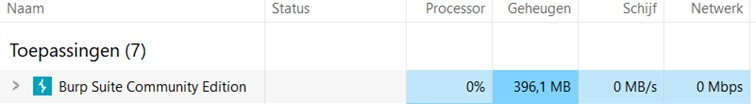
\includegraphics[height=0.1\textheight]{Burp_suite_rust.jpg}
    \caption[Resource gebruik van Burp suite in rust]{Resource gebruik van Burp suite in rust}
    \label{fig:burp_suite_rust}
\end{figure}
\begin{figure}
    \centering
    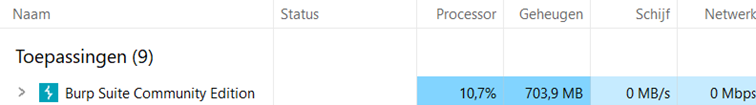
\includegraphics[height=0.1\textheight]{burp_suite_in_actie.png}
    \caption[Resource gebruik van Burp suite tijdens het uitvoeren van een actie]{Resource gebruik van Burp suite tijdens het uitvoeren van een actie}
    \label{fig:burp_suite_actie}
\end{figure}
\begin{figure}
    \centering
    
\includegraphics[height=0.025\textheight]{Metasploit_rust.png}
    \caption[Resource gebruik van Metasploit in rust]{Resource gebruik van Metasploit in rust}
    \label{fig:metasploit_rust}
\end{figure}
\begin{figure}
    \centering
    
\includegraphics[height=0.02\textheight]{Metasploit_in_actie.png}
    \caption[Resource gebruik van Metasploit tijdens het uitvoeren van een actie]{Resource gebruik van Metasploit tijdens het uitvoeren van een actie}
    \label{fig:metasploit_actie}
\end{figure}
\begin{figure}
    \centering
    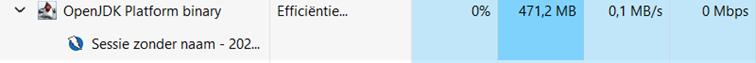
\includegraphics[height=0.05\textheight]{OWASP_ZAP_rust.png}
    \caption[Resource gebruik van OWASP ZAP in rust]{Resource gebruik van OWASP ZAP in rust}
    \label{fig:owasp_rust}
\end{figure}
\begin{figure}
    \centering
    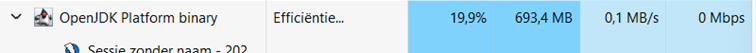
\includegraphics[height=0.05\textheight]{OWASP_ZAP_in_actie.png}
    \caption[Resource gebruik van OWASP ZAP tijdens het uitvoeren van een actie]{Resource gebruik van OWASP ZAP tijdens het uitvoeren van een actie}
    \label{fig:owasp_actie}
\end{figure}
Om het resourcegebruik van de drie pentesting-tools te vergelijken, wordt zowel het verbruik in rust als het verbruik tijdens het 
uitvoeren van een actie gemeten. De eerste tool waarvan het resourcegebruik is gemeten is Burp Suite. Hierbij zijn zowel de 
prestaties in rust als tijdens actieve taken geregistreerd. De resultaten van deze metingen zijn te zien in de afbeeldingen. 
Dit is in rust \ref{fig:burp_suite_rust} en dit is tijdens het uitvoeren van een actie \ref{fig:burp_suite_actie}. 

Voor het vergelijken van het resourcegebruik is ook Metasploit onderworpen aan metingen in zowel rust als tijdens actieve 
penetratietests. Metasploit wordt uitgevoerd in de terminal, daarom zijn de resource resultaten te zien onder de terminal tab 
in taakbeheer. Deze metingen geven inzicht in de efficiëntie van Metasploit onder verschillende omstandigheden. De 
resultaten van het resourcegebruik in rust zijn te vinden in figuur \ref{fig:metasploit_rust}, terwijl het verbruik tijdens 
actieve testen wordt weergegeven in figuur \ref{fig:metasploit_actie}.

OWASP ZAP is eveneens geanalyseerd op zijn resourcegebruik, zowel in rust als tijdens het uitvoeren van beveiligingstests. 
Deze metingen helpen bij het bepalen van de belasting die ZAP op het systeem legt onder verschillende operationele scenario's. 
De resultaten van het resourcegebruik van OWASP ZAP in rust zijn weergegeven in figuur \ref{fig:owasp_rust}, en tijdens het 
uitvoeren van acties in figuur \ref{fig:owasp_actie}.

\subsubsection{\IfLanguageName{dutch}{Ondersteuning van de community }{Ondersteuning van de community}}
\begin{figure}
    \centering
    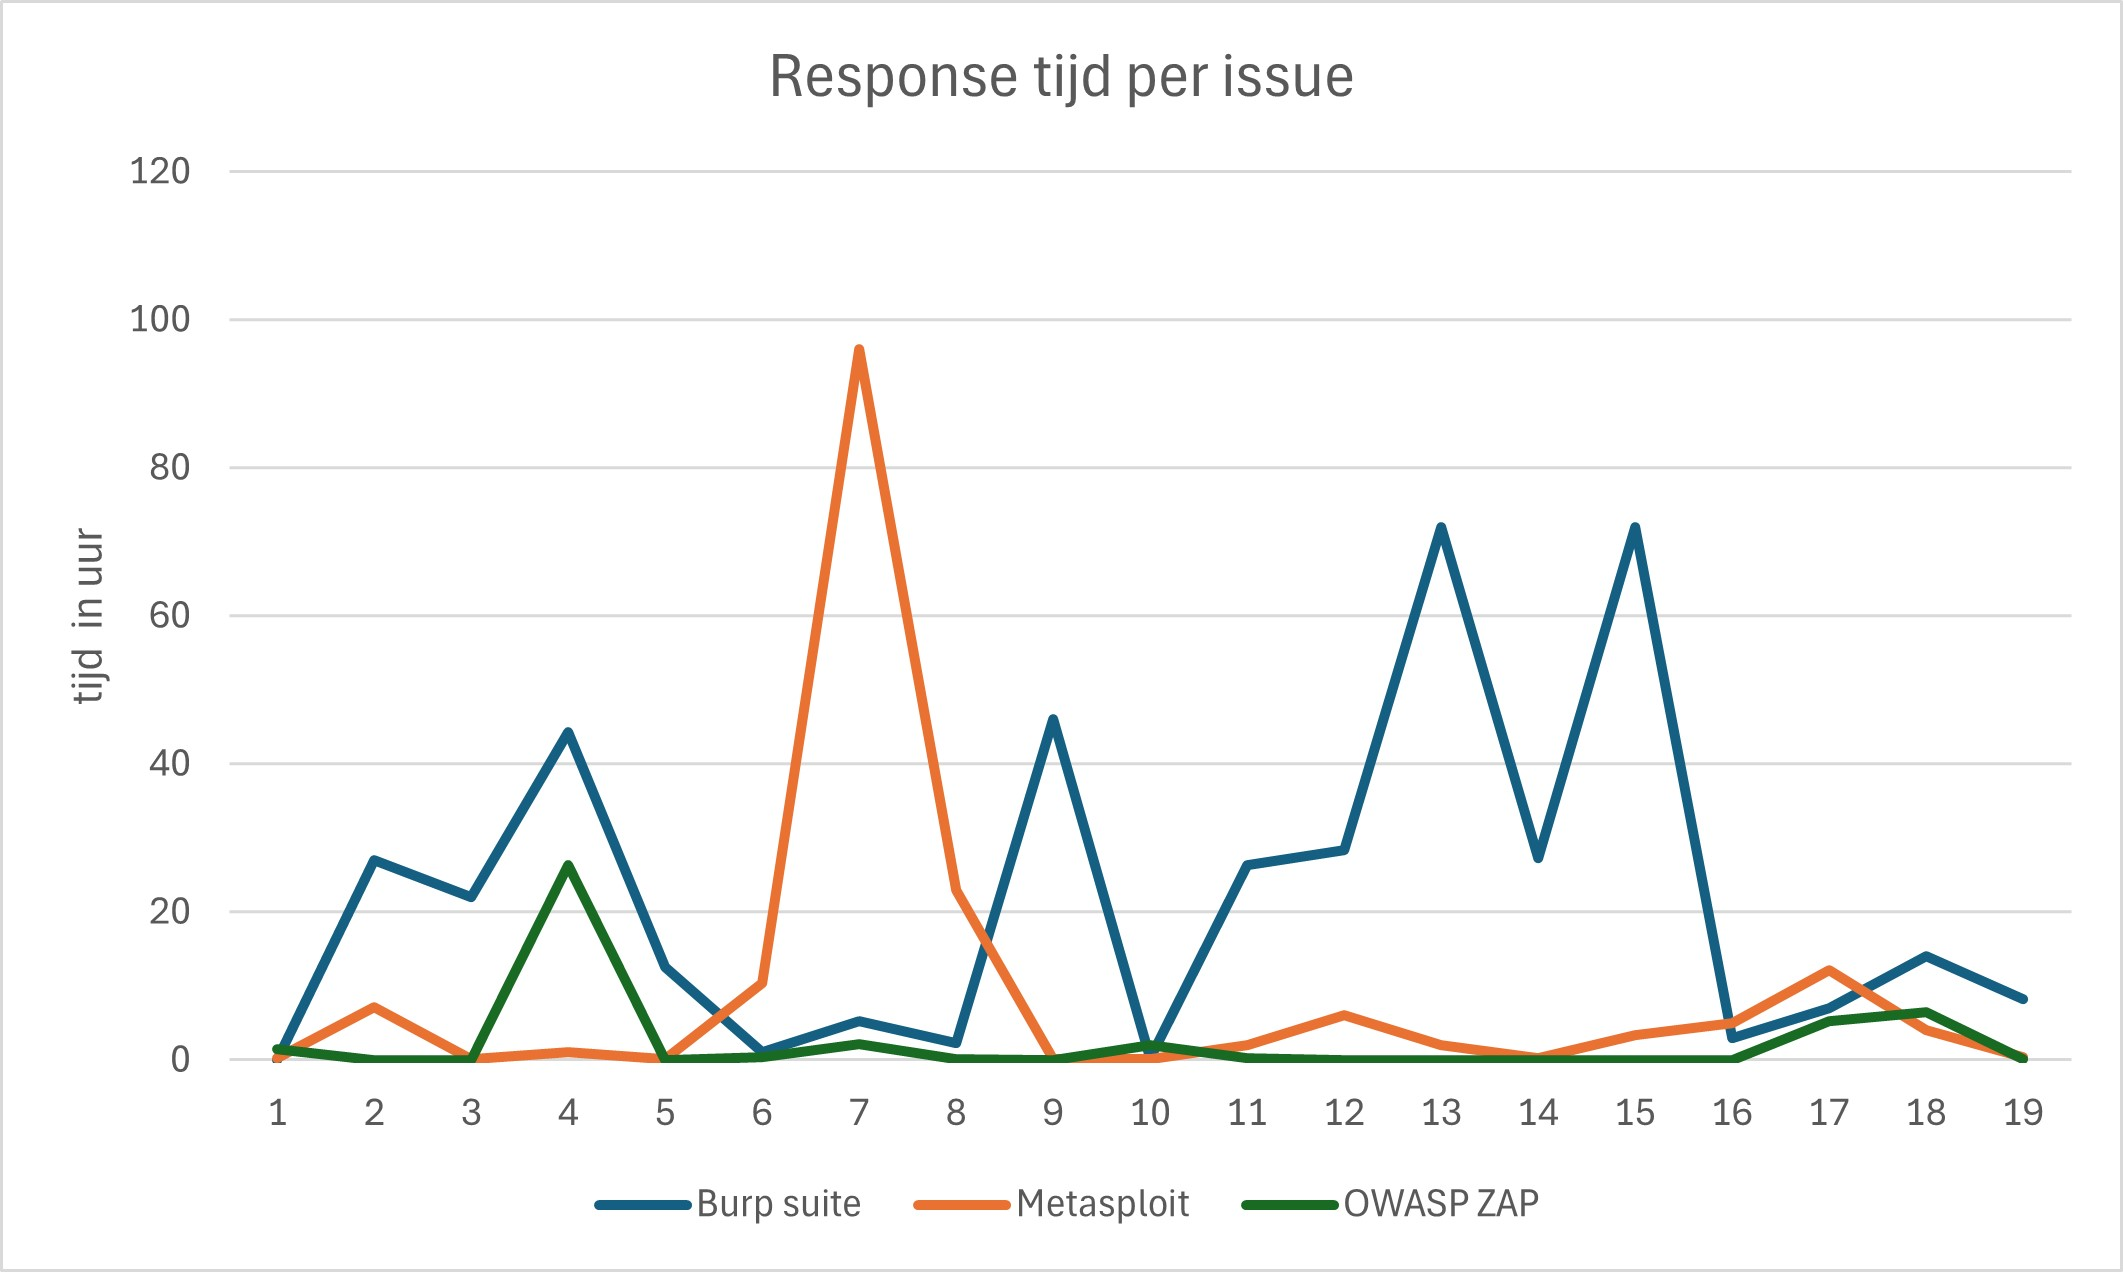
\includegraphics[height=0.3\textheight]{grafiek_respons_resultaten.jpg}
    \caption[Grafiek van 19 willekeurige issues bij de pentesttools en de tijd hoe lang het duurt om te repliceren]{Grafiek van 19 willekeurige issues bij de pentesttools en de tijd hoe lang het duurt om te repliceren}
    \label{fig:respons_grafiek}
\end{figure}
De ondersteuning van de developers of de community is een belangrijke factor bij het kiezen van een pentesting-tool. Om de ondersteuning 
te evalueren, zijn 19 willekeurige issues gemeld bij de drie pentesting-tools. De tijd die nodig is om deze
vragen te beantwoorden, is vastgelegd en geanalyseerd. De resultaten van deze analyse zijn te zien in de
grafiek \ref{fig:respons_grafiek}. Hieruit blijkt dat OWASP ZAP de snelste responstijd heeft, gevolgd door Metasploit en
Burp Suite. Dit zijn de gemiddelde response tijden van de 19 issues die zijn gemeld bij de drie pentesting-tools.
\begin{itemize}
    \item OWASP ZAP: 2u 46 min
    \item Metasploit: 8u
    \item Burp Suite: 22u 15 min
\end{itemize}

Aangezien OWASP ZAP en Metasploit open-source tools zijn, zijn de issues te vinden op github en is de community actief
betrokken bij het oplossen van problemen. Burp Suite is een commerciële tool en heeft een eigen support team dat 
verantwoordelijk is voor het oplossen van problemen. In tegenstelling tot Metasploit en OWASP ZAP worden de issues niet 
op github gepost, maar op een apart platform portswigger. Dit kan de responstijd beïnvloeden, 
aangezien de issues eerst opgepakt moeten worden door het support team.

\subsubsection{\IfLanguageName{dutch}{Globale resultaten}{Global results}}
Na het analyseren van de capaciteiten en functionaliteiten, het resourcegebruik en de ondersteuning van de community,
kunnen de resultaten van de drie pentesting-tools worden samengevat. De vergelijking van de drie tools toont aan dat
OWASP ZAP de meest uitgebreide functionaliteiten biedt voor het testen van webapplicaties, gevolgd door Burp Suite 
community edition en Metasploit. 

De resultaten van de resource metingen tonen aan dat Metasploit het minste 
geheugen en CPU verbruikt in vergelijking met Burp Suite en OWASP ZAP. Het verbruik van OWASP ZAP ligt iets hoger dan 
Burp Suite, maar is nog steeds acceptabel voor de meeste systemen. 

De responstijd van de community is het snelst bij OWASP ZAP, 
gevolgd door Metasploit en Burp Suite. Dit toont aan dat OWASP ZAP de meest actieve community heeft die snel reageert op 
gemelde problemen.

Deze resultaten bieden een overzicht van de prestaties van de drie pentesting-tools en helpen bij het bepalen van de 
meest geschikte tool voor het uitvoeren van beveiligingstests op webapplicaties. Op basis van deze resultaten kan een 
definitieve conclusie worden getrokken over welke tool het meest geschikt is voor de tests. Volgens de eigen criteria 
lijkt OWASP ZAP de beste keuze te zijn voor het uitvoeren van beveiligingstests op webapplicaties, gevolgd door Burp Suite 
community edition en Metasploit. 

\subsection{\IfLanguageName{dutch}{Resultaat volgens derden}{Result with third parties}}
Na de vergelijking van de drie pentesting-tools volgens de eigen criteria, worden de resultaten getoetst aan bevindingen van 
derden.

De resultaten van externe gebruikers worden bepaald door drie factoren te analyseren: voordelen, nadelen en een algemene 
beoordeling van elke tool. Deze factoren trachten inziecht te bieden in de ervaringen van andere gebruikers met de drie pentesting-tools. 
De bevindingen van derden worden gebruikt om de betrouwbaarheid van de eigen resultaten al dan niet te bevestigen en een definitieve conclusie 
te trekken om één tool te weerhouden voor de tests.

De voordelen van Burp Suite betreffen het gebruiksgemak en de gebruiksvriendelijke interface. De nadelen zijn echter 
de hoge kosten van de Professional Edition, de beperkte functionaliteiten in de Community Edition en de trage prestaties. De 
algemene beoordeling van Burp Suite community edition komt uit op 4,8/5.

OWASP ZAP wordt gewaardeerd om zijn gebruiksvriendelijkheid, uitgebreide automatiseringsmogelijkheden en efficiëntie. Aan de 
andere kant zijn de nadelen de beperkte documentatie en de gelimiteerde scope van de tool. De algemene beoordeling van OWASP 
ZAP is 4,7/5.

Metasploit staat bekend om zijn efficiëntie en kwalitatieve resultaten. Echter, de tool wordt ook als complex ervaren en 
heeft een steile leercurve, wat een uitdaging kan zijn voor minder ervaren gebruikers. De algemene beoordeling van Metasploit 
is 4,6/5.

\subsection{\IfLanguageName{dutch}{Definitieve pentesttool}{}}
Na het analyseren van de resultaten van derden en de opgestelde criteria, blijkt dat OWASP ZAP de best passende tool is voor het uitvoeren van 
beveiligingstests op webapplicaties binnen de context van een KMO webdeveloper zoals Sinergio. De tool biedt een uitgebreide reeks functionaliteiten en is gebruiksvriendelijk, wat 
het een aantrekkelijke keuze maakt voor organisaties die op zoek zijn naar een kosteneffectieve oplossing voor het uitvoeren 
van beveiligingstests. Ook de automatiseringsmogelijkheden en efficiëntie van OWASP ZAP dragen bij aan de positieve 
beoordeling van de tool.

\section{\IfLanguageName{dutch}{Resultaten van webomgevingen}{Results of web environments}}
\subsection{\IfLanguageName{dutch}{Wordpress CMS-framework resultaten}{Wordpress CMS-framework results}}
\subsection{\IfLanguageName{dutch}{Laravel resultataten}{Laravel results}}


\begin{comment}
\section{\IfLanguageName{dutch}{Brute Force Attack op WordPress Omgevingen met Beveiligingsplugins}{Brute Force Attack on WordPress enviroment with securityplugins}}
Binnen de context van webbeveiliging zijn brute force aanvallen een veelvoorkomende methode waarbij aanvallers trachten toegang te krijgen tot een systeem 
door herhaaldelijk logins of wachtwoorden te raden. Dit type aanval kan bijzonder schadelijk zijn voor systemen zoals WordPress, die veel 
gebruikt worden voor het bouwen van websites.In dit hoofdstuk onderzoeken we de effectiviteit van verschillende penetratietesttools bij het uitvoeren van 
brute force aanvallen op een WordPress-omgeving beveiligd met de Wordfence plugin. Het doel is niet om de beveiligingsplugins zelf te testen, maar om de 
prestaties, de mogelijkheden en bruikbaarheid van de tools Burp Suite, Metasploit en OWASP ZAP met elkaar te vergelijken. Deze analyse zal helpen vaststellen welke tool 
het meest effectief en gebruiksvriendelijkst is voor het tonen van kwetsbaarheden in een beschermde WordPress-omgeving.

\subsection{\IfLanguageName{dutch}{Resultaat met burp suite}{result with burp suite}}
\begin{figure}
    \centering
    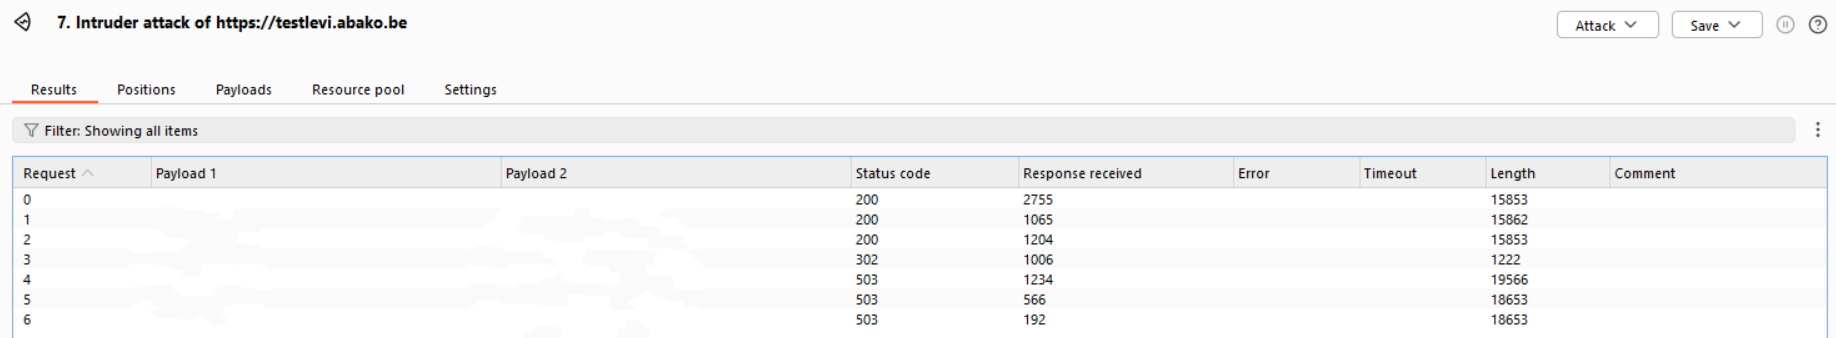
\includegraphics[height=0.1\textheight]{burp-suite_bruteforce_wordpressplugins_blurred.png}
    \caption[Burp suite brute force attack op wordpress applicatie met beveiligingsplugin]{Burp suite brute force attack op wordpress applicatie met beveiligingsplugin}
\end{figure}
De brute force attack op een WordPress omgeving met wordfence beveiligingsplugin werd uitgevoerd met behulp van Burp Suite Community Edition. Tijdens de test viel het 
op dat enkele functionaliteiten beperkt waren vanwege de beperkingen van de Community Edition. Dit beperkte de mogelijkheden van het uitvoeren van een volledige 
pentest, maar het voordeel van Burp Suite is dat er veel documentatie en tutorials beschikbaar zijn op het internet, wat nuttig kan zijn bij het oplossen van 
eventuele problemen tijdens het gebruik van de tool.

Naast de brute force attack werd er ook een SQL-injectie pentest uitgevoerd met Burp Suite. In de WordPress-omgeving met beveiligingsplugins werd de SQL-injectie aanval 
effectief gedetecteerd en geblokkeerd door de beveiligingsmaatregelen van Wordfence. Dit toont aan dat de plugins niet alleen bescherming bieden tegen brute force 
aanvallen, maar ook tegen SQL-injecties, wat cruciaal is voor de algehele beveiliging van de applicatie

\subsection{\IfLanguageName{dutch}{Resultaat met metasploit}{result with metasploit}}
\begin{figure}
    \centering
    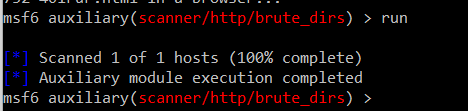
\includegraphics[height=0.1\textheight]{metasploit_brute_wordpressplugin.png}
    \caption[Metasploit brute force attack op wordpress applicatie met beveiligingsplugin]{Metasploit brute force attack op wordpress applicatie met beveiligingsplugin}
\end{figure}
Metasploit is een populair open-source framework voor beveiligingstests, dat vooral wordt ingezet voor het ontwikkelen en implementeren van exploit-codes. 
Met dit framework kunnen systemen worden beoordeeld op veiligheid door actief kwetsbaarheden te exploiteren en te identificeren. 
Metasploit beschikt over honderden exploit-modules die een breed scala aan bekende kwetsbaarheden dekken, waardoor het als een belangrijk 
instrument kan worden gezien in de toolkit van veel cybersecurity-professionals.

In een praktische toepassing werd Metasploit gebruikt om een brute force attack uit te voeren op een WordPress-omgeving die beveiligd was met de Wordfence plugin. 
Voor deze test diende de tool via de terminal bediend worden. Hoewel dit als een beperking kan worden gezien, biedt Metasploit een uitgebreid scala aan 
mogelijkheden voor het uitvoeren van penetratietests. De tool stelt gebruikers in staat om diverse aanvalsscenario's te simuleren en levert een uitgebreide reeks 
modules voor het uitvoeren van verschillende soorten beveiligingstests. Deze flexibiliteit en diepgang maken van Metasploit een waardevolle keuze voor professionals die 
uitgebreide beveiligingstests willen uitvoeren op complexe netwerken en systemen.

\subsection{\IfLanguageName{dutch}{Resultaat met OWASP ZAP}{result with OWASP ZAP}}
\begin{figure}
    \centering
    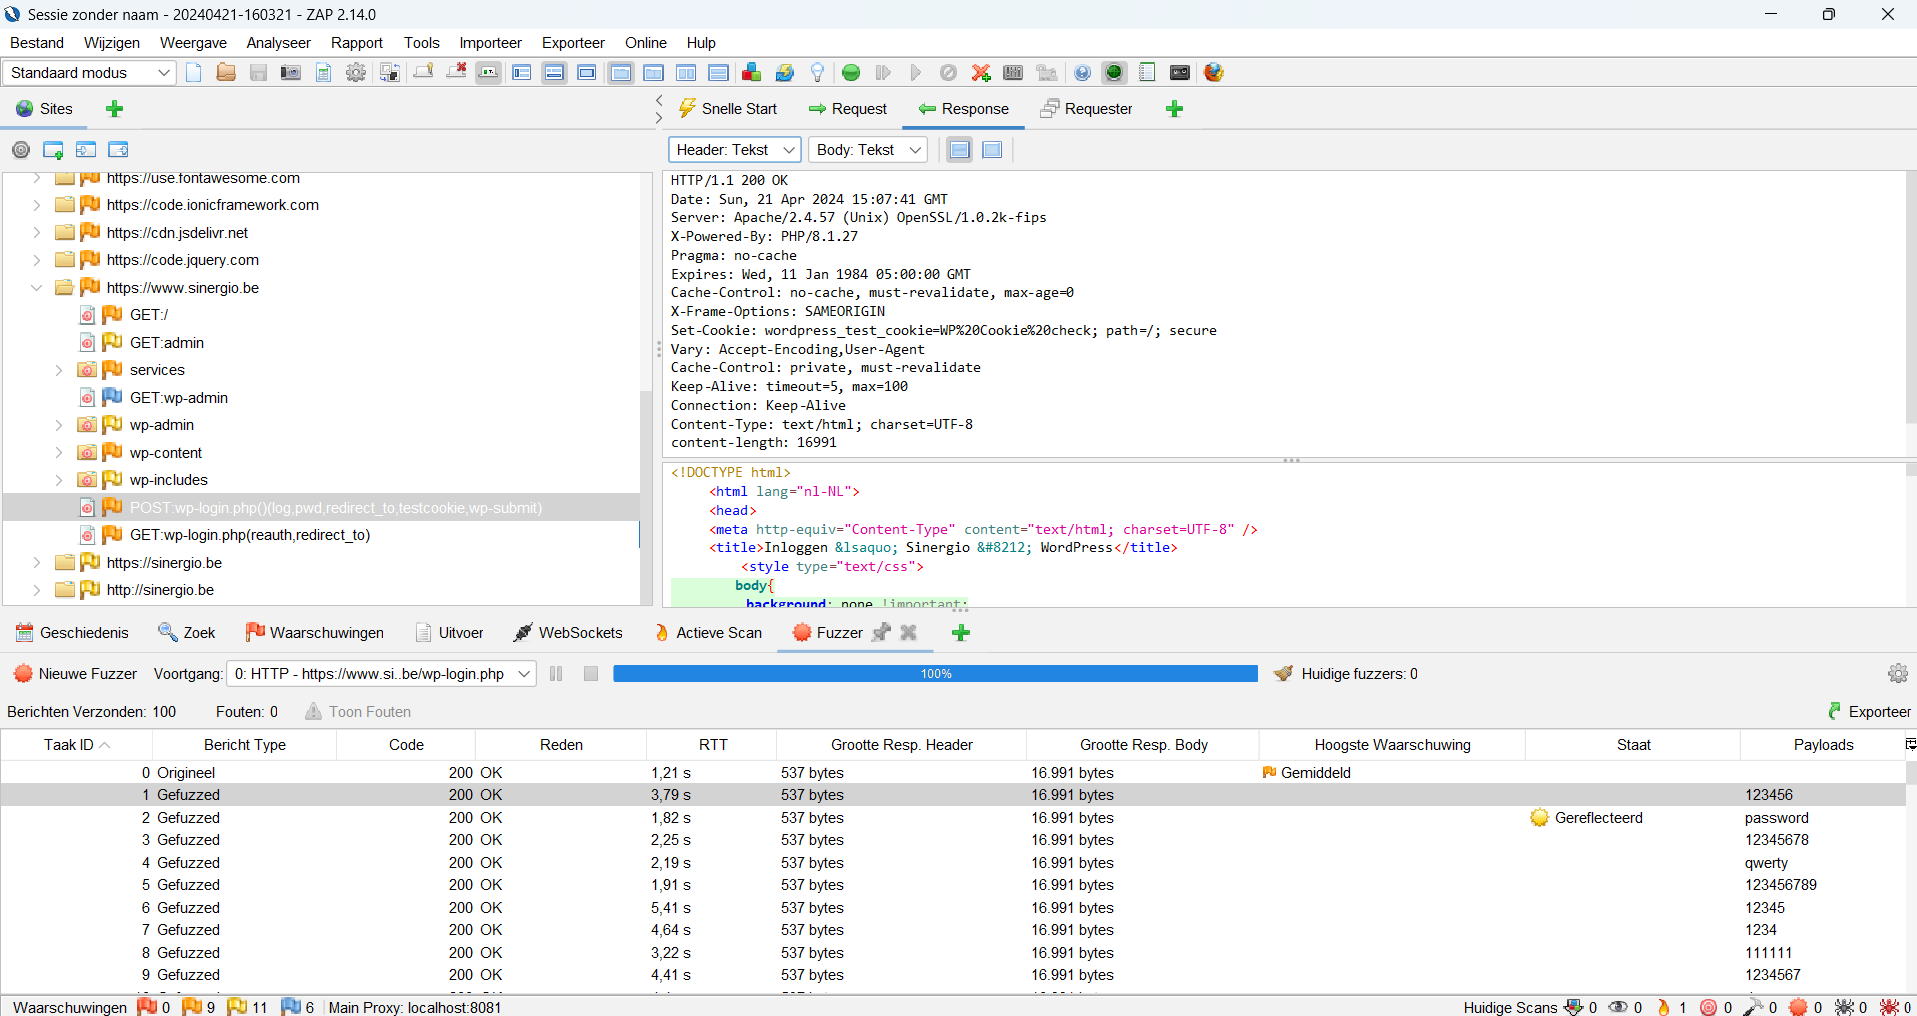
\includegraphics[height=0.3\textheight]{ZAP_brute_wordpressplugin.png}
    \caption[OWASP ZAP brute force attack op wordpress applicatie met beveiligingsplugin]{OWASP ZAP brute force attack op wordpress applicatie met beveiligingsplugin}
\end{figure}

Voor de brute force attack op de WordPress omgeving met wordfence werd OWASP ZAP gebruikt, een open source tool die bekend staat om zijn gebruiksgemak. 
Wat opviel bij het gebruik van OWASP ZAP was dat de resultaten van de testen vergelijkbaar waren als bij de betalende Burp Suite, maar dan met een open source alternatief. 
Dit maakt van OWASP ZAP een aantrekkelijke keuze voor organisaties die op zoek zijn naar een kosteneffectieve oplossing voor het uitvoeren van beveiligingstests.

Daarnaast werd met OWASP ZAP ook een SQL-injectie pentest uitgevoerd. De beveiligingsplugin van WordPress detecteerde en blokkeerde de SQL-injectie aanval effectief, 
wat wederom de betrouwbaarheid van de beveiligingsmaatregelen aantoont. OWASP ZAP's intuïtieve interface en effectieve testresultaten maken het een sterke concurrent 
voor andere penetratietesttools. Een voorbeeld van deze pentest kan hier worden teruggevonden \ref{fig:sql-injection}.

\section{\IfLanguageName{dutch}{Vergelijking van omgevingen}{Comparison of environments}}
%\begin{figure}
%    \centering
%    \includegraphics[height=0.1\textheight]{ }
%    \caption[Brute force aanval op een wordpress applicatie zonder beveiligingsplugins (foto moet nog geblurred worden)]{Brute force aanval op een wordpress site zonder beveiligingsplugins}
%\end{figure}
\subsection{\IfLanguageName{dutch}{WordPress Zonder Beveiligingsplugins}{WordPress without securityplugins}}
De eerste testomgeving was een standaard WordPress-applicatie zonder enige vorm van beveiligingsplugins. De resultaten toonden aan dat deze 
omgeving bijzonder kwetsbaar was voor brute force aanvallen. Aanvallers zijn in staat om binnen enkele minuten toegang te verkrijgen door middel 
van standaard gebruikersnamen zoals 'admin' en algemeen bekende zwakke wachtwoorden. Deze bevindingen benadrukken de noodzaak voor 
basisbeveiligingsmaatregelen, zoals het instellen van sterke wachtwoorden en het gebruik van moeilijkere gebruikersnamen om de initiële 
beveiliging te verstevigen.

\begin{figure}
    \centering
    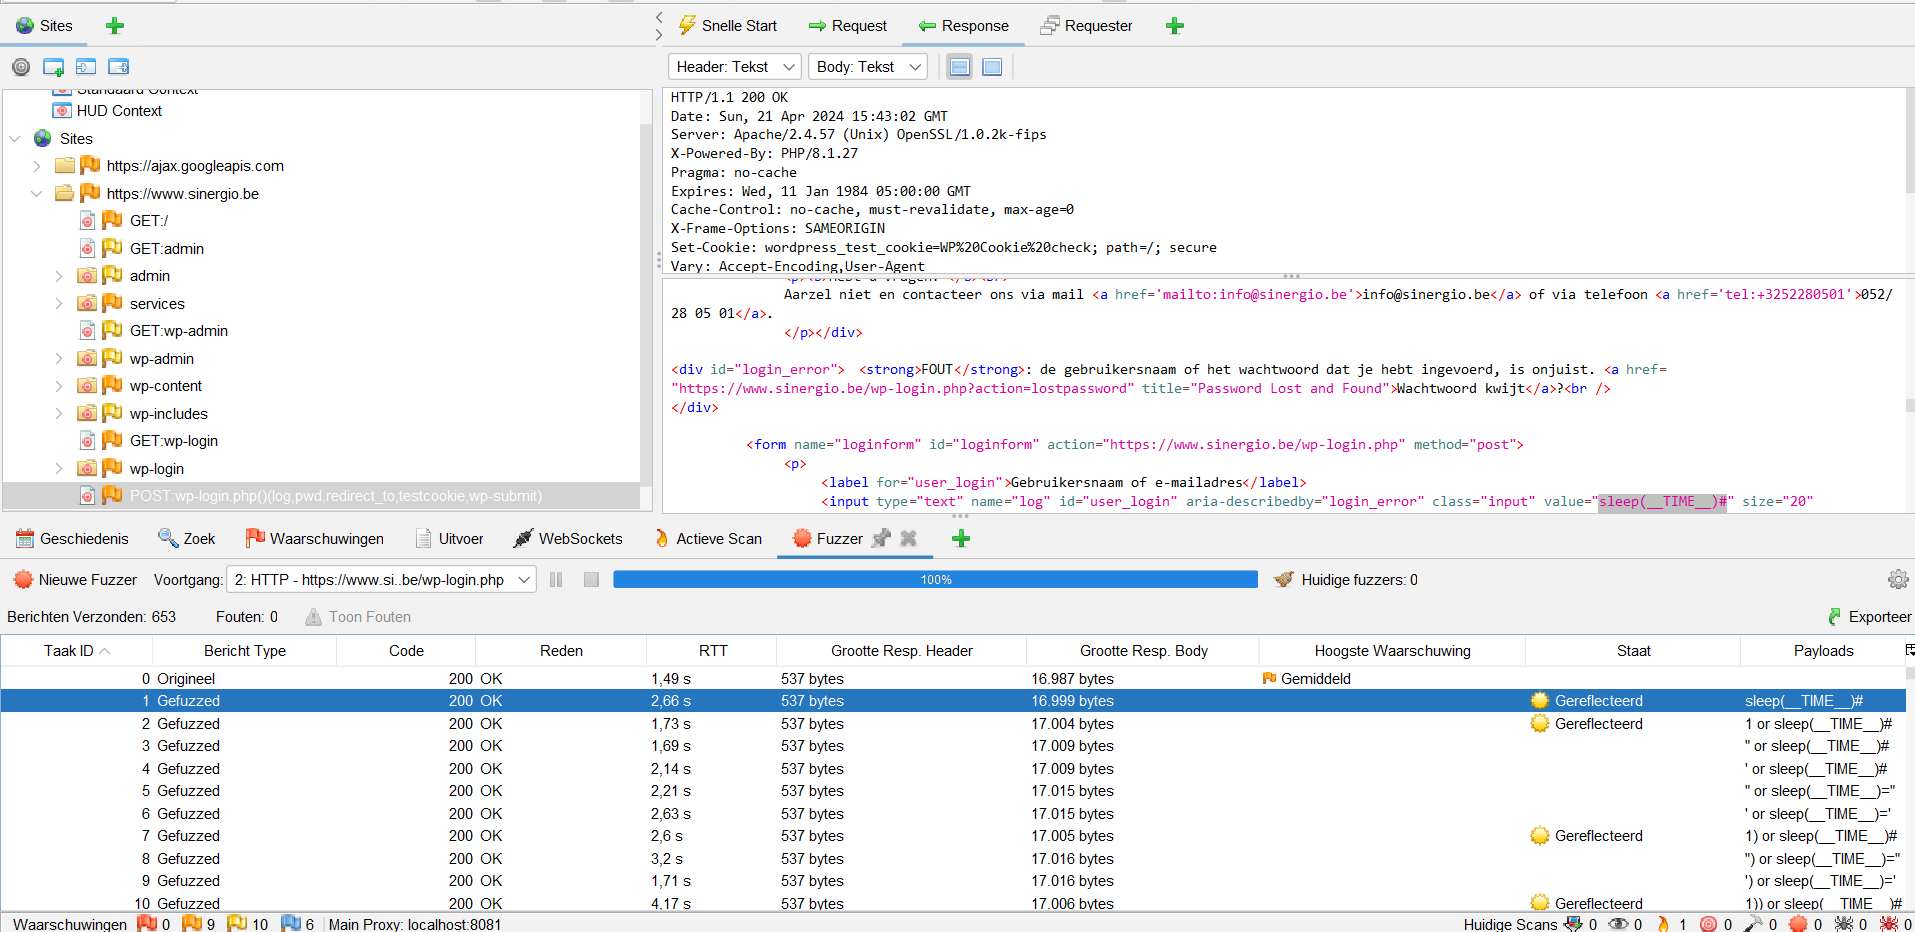
\includegraphics[height=0.2\textheight]{zap_sql-injection_wordpressplugin.png}
    \caption[SQL-injection aanval op een wordpress applicatie met beveiligingsplugins]{SQL-injection aanval op een wordpress applicatie met beveiligingsplugins}
    \label{fig:sql-injection}
\end{figure}
\subsection{\IfLanguageName{dutch}{WordPress Met Beveiligingsplugins}{WordPress with securityplugins}}
De tweede test-omgeving, een WordPress-installatie uitgerust met specifieke beveiligingsplugins zoals Wordfence, liet een aanzienlijke 
verbetering zien in beveiliging tegen brute force-aanvallen. De plugins die werden getest, bieden functionaliteiten zoals limieten 
op inlogpogingen, directe accountvergrendeling bij verdachte activiteiten en real-time monitoring en alerts. Deze maatregelen 
leiden tot een snelle detectie en blokkering van aanvalspogingen, waardoor de veiligheid van de omgeving aanzienlijk werd verhoogd.

\begin{figure}
    \centering
    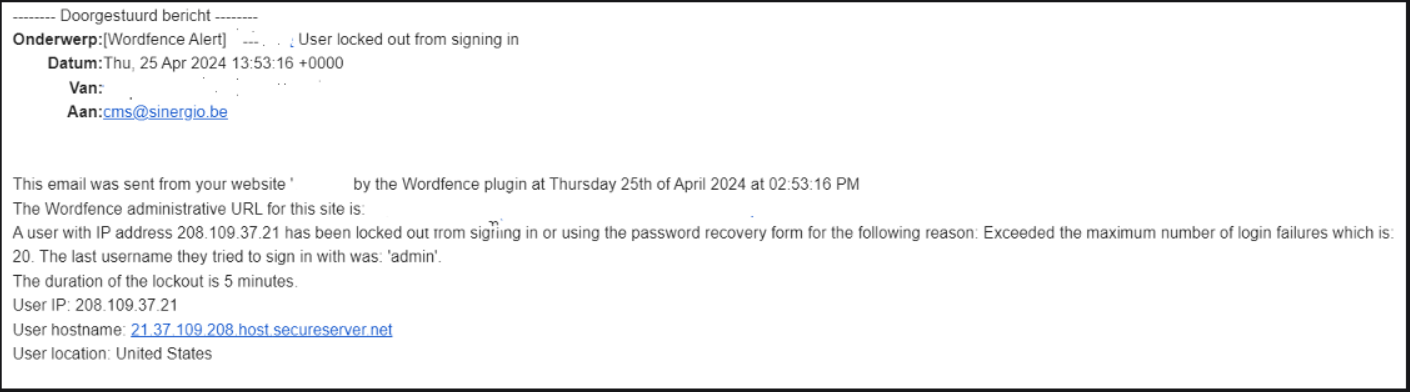
\includegraphics[height=0.2\textheight]{foute_login_mail_blurred.png}
    \caption[E-mail over geblokkeerde inlog poging]{E-mail over geblokkeerde inlog poging}
    \label{fig:geblokkeerde-login}
\end{figure}
Wanneer een gebruiker bijvoorbeeld het maximum aantal mislukte inlogpogingen overschrijdt, stuurt Wordfence een alert. 
Een typische melding kan er als volgt uitzien: "A user with IP address 208.109.37.21 has been locked out from signing in or 
using the password recovery form for the following reason: Exceeded the maximum number of login failures which is: 20. The 
last username they tried to sign in with was: 'admin'. The duration of the lockout is 5 minutes."

Deze melding bevat belangrijke informatie zoals:
\begin{itemize}
    \item IP-adres van de aanvaller: In dit geval 208.109.37.21.
    \item Hostname: 21.37.109.208.host.secureserver.net.
    \item Locatie van de gebruiker: United States.
    \item Gebruikersnaam: De laatste gebruikersnaam waarmee geprobeerd werd in te loggen, bijvoorbeeld 'admin'.
    \item Reden voor blokkering: Het overschrijden van het maximum aantal mislukte inlogpogingen, hier vastgesteld op 20.
    \item Duur van de blokkering: In dit geval 5 minuten.
\end{itemize}
Als deze limiet is bereikt, ontvang je een vergelijkbare alert met details over de geblokkeerde gebruiker en de 
blokkeringstijd.

Verder biedt Wordfence ook directe accountvergrendeling bij verdachte activiteiten. Dit blokkeert onmiddellijk een 
account wanneer bijvoorbeeld een plotseling groot aantal mislukte inlogpogingen wordt gedetecteerd. De alert geeft 
aan welk account is vergrendeld en de reden voor de vergrendeling.

Wordfence biedt daarnaast real-time monitoring van je website, waarbij verdachte activiteiten direct worden gemeld. 
Deze alerts kunnen variëren van verdachte inlogpogingen tot pogingen om kwetsbaarheden in plugins of thema's te misbruiken.
Een voorbeeld van een dergelijke alert kan je hier zien \ref{fig:geblokkeerde-login}. 

Deze resultaten onderstrepen het belang van het toepassen van gespecialiseerde beveiligingsuitbreidingen in populaire 
CMS-systemen, wat aantoont dat zelfs fundamentele beveiligingsplugins een significante bescherming kunnen bieden.
\begin{figure}
    \centering
    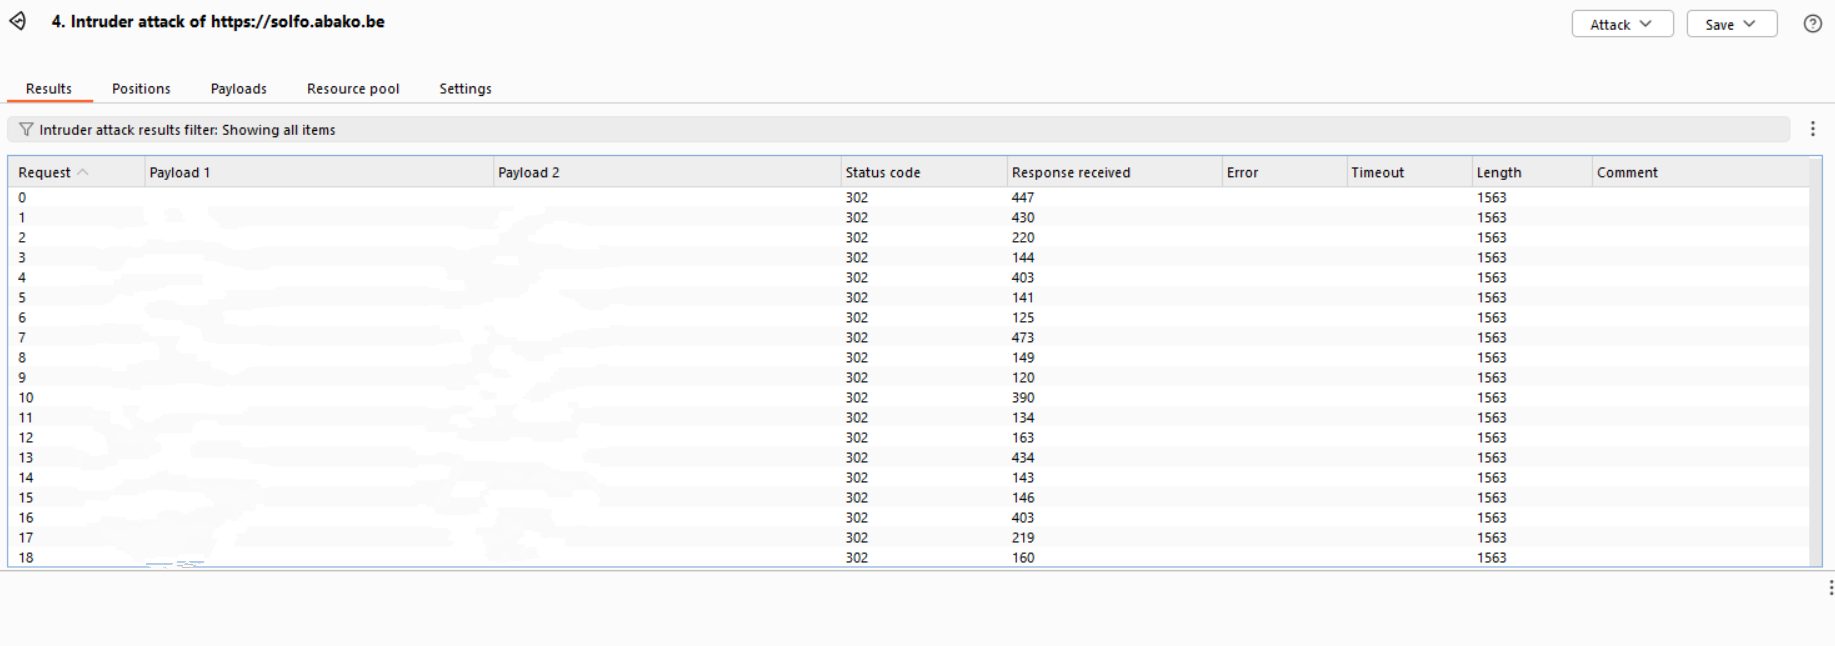
\includegraphics[height=0.2\textheight]{burp-suite_bruteforce_laravel_blurred.png}
    \caption[Brute force aanval op een laravel applicatie]{Brute force aanval op een laravel applicatie}
    \label{fig:laravel-brute-force}
\end{figure}
\subsection{\IfLanguageName{dutch}{Laravel Applicatie}{Laravel Application}}
Na de aanval analyseerden we de resultaten. Er werden geen succesvolle inlogpogingen gedetecteerd zoals je kan zien op foto \ref{fig:laravel-brute-force}, wat erop wijst dat de 
gebruikersnamen en wachtwoorden sterk genoeg waren om brute force aanvallen te weerstaan. Bovendien reageerde het systeem 
effectief op de aanvalspogingen door IP-adressen te blokkeren en CAPTCHA's te tonen. Een CAPTCHA is zijn een reactietest 
die in de gegevensverwerking wordt gebruikt om te bepalen of er al dan niet sprake is van een menselijke gebruiker. Dit toont aan dat er goede 
beveiligingsmaatregelen zoals account lockout policies en rate limiting waren geïmplementeerd.

In ons gedetailleerde rapport beschreven we de methodologie, de gebruikte tools, de configuraties, en de uitkomsten van de 
test. Hoewel de brute force aanval niet succesvol was, benadrukten we het belang van continue beveiligingsmonitoring en 
periodieke tests om de beveiliging up-to-date te houden. We gaven aanbevelingen zoals het blijven versterken van het 
wachtwoordbeleid, het implementeren van multi-factor authenticatie (MFA) voor extra beveiligingslagen, en het gebruik 
van intrusion detection en prevention systems (IDPS) om ongeautoriseerde toegangspogingen vroegtijdig te detecteren en 
te stoppen.
\end{comment}